\begin{section}{SS}{Incorporating the Cosmological Radiative Transfer code, \\
    \hspace*{4cm} RADAMESH with Hydrodynamics}{(Saeed Sarpas, PhD)}
  \begin{minipage}{\linewidth}
    \strut {\small The advent of supercomputers and more efficient CPU
      architectures has enabled cosmologists to simulate the Universe in more
      detail. So far, Gravity, Hydrodynamics and radiative cooling and heating
      effects have been included into cosmological simulations, however
      still some important parts of the puzzle (such as
      proper stellar and AGN feedback mechanisms, magneto-hydrodynamics and
      radiative transfer effects) are either missing or not fully implemented.
      In the era of high precision cosmology, adding these extra phenomena to
      cosmological simulation seems crucial,
      especially to reach percent accurate results. Our objective is to
      incorporate the cosmological radiative transfer code (RADAMESH) with
      hydrodynamics.
      Presently, these effects are treated in a post-processing state.
      Considering the active role of radiative hydrodynamics in cosmic structure
      formation, post-processing these effects might lead to less accurate
      results. The
      non-local nature of radiative transfer effects make them extremely tricky and
      challenging to be implemented in an efficient way. We accept this
      challenge with the expectation of getting more precise results especially
      in the environment of our interest which is circumgalactic medium
      (CGM) illuminated by a bright quasar.\\
      The pictures show how a bright quasar is able to ionize its
      environment in a comparably short period of time (here the interval
      between two snapshots is less than 0.1 Myr). This
      result has been generated by post-processing an EAGLE snapshot at z
      $\approx$ 3 using RADAMESH code.
    }
  \end{minipage}

  \vspace{0.5cm}

  \begin{minipage}{\linewidth}
    \begin{center}
      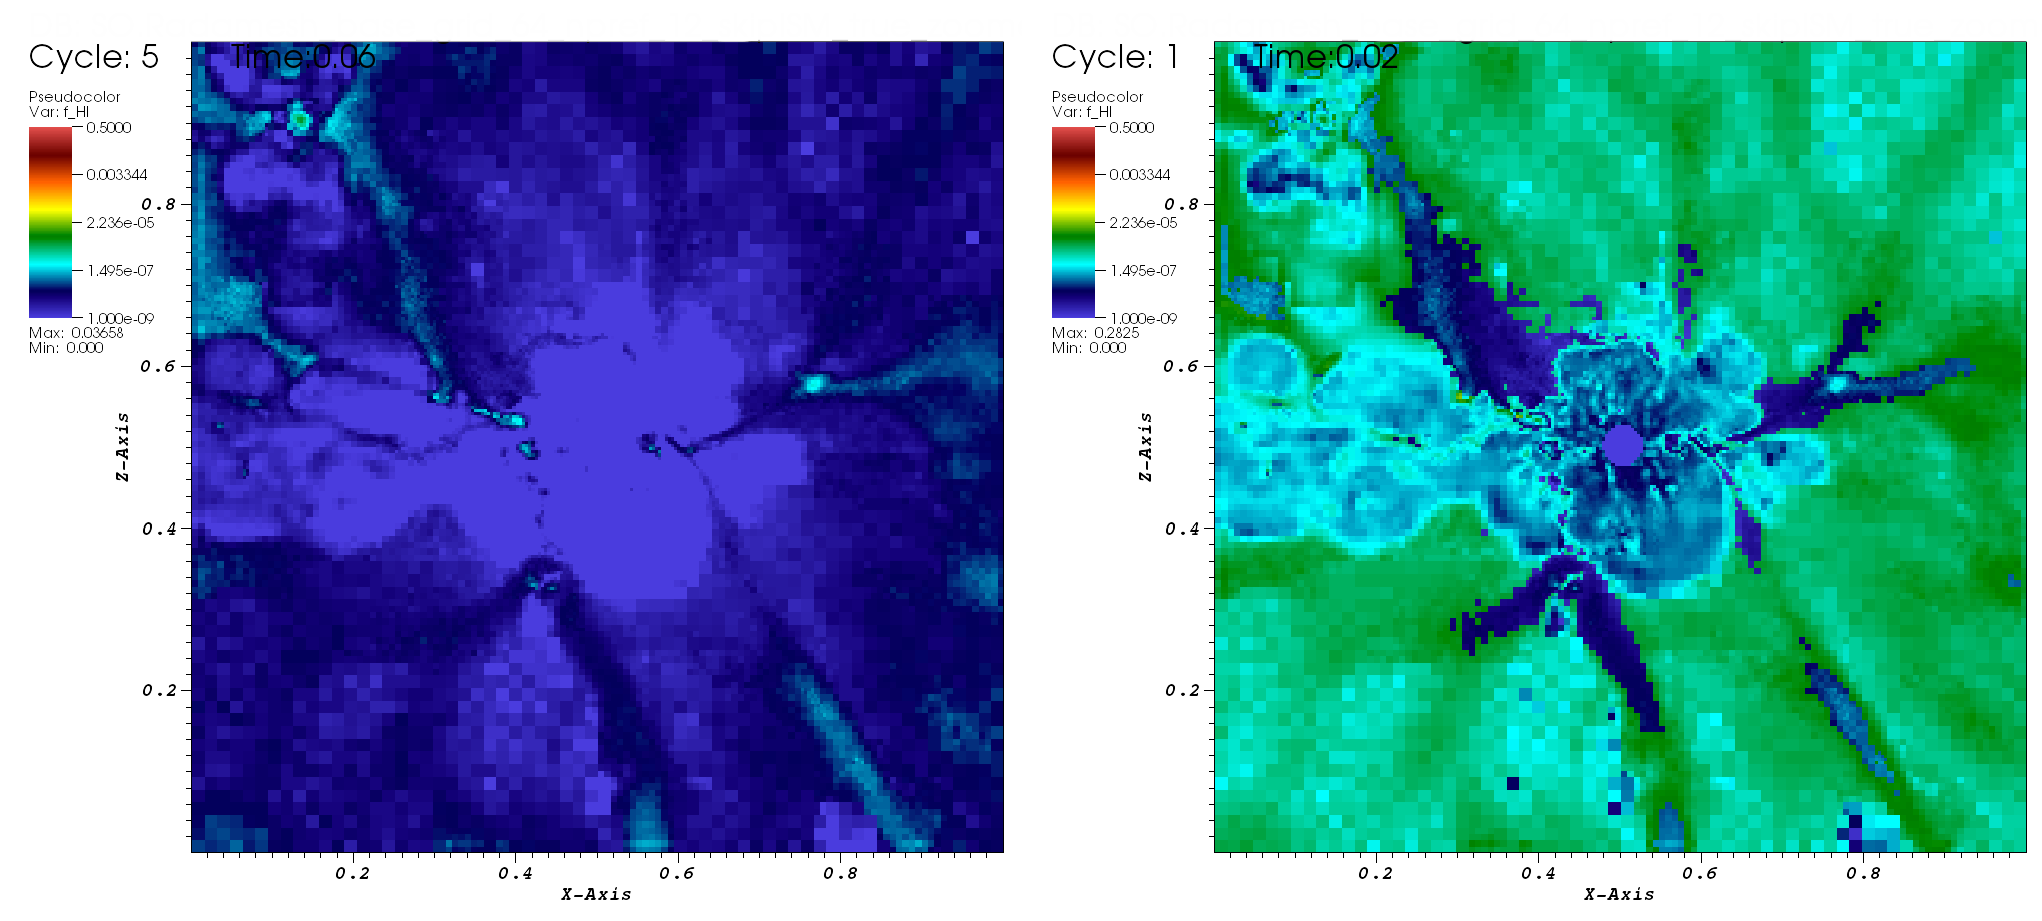
\includegraphics[height=10cm]{SS/QSO.png}
    \end{center}
  \end{minipage}
\end{section}